\documentclass{assignment}
\usepackage{float}
\usepackage{gensymb}
\usepackage{parskip}
\usepackage{amsmath}
\begin{document}

\assignmentTitle{mcgill_logo.jpg}{Homework 2}{Gian Favero | 261157396}{ECSE 556}{December 1st, 2023}

\section{Some Graph Theory}
We can consider a simple graph network to help facilitate the proof:
\begin{figure}[H]
    \centering
    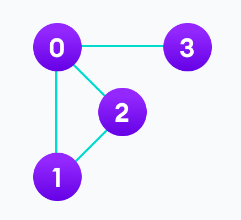
\includegraphics[width=0.25\textwidth]{LaTeX Images/UUG.png}
    \caption{A simple undirected graph}
    \label{fig:my_label}
\end{figure}

This graph has a corresponding adjacent matrix:
\begin{align*}
    A = \begin{bmatrix}
        0 & 1 & 1 & 1 \\
        1 & 0 & 1 & 0 \\
        1 & 1 & 0 & 0 \\
        1 & 0 & 0 & 0 \\
    \end{bmatrix}
\end{align*}

We can prove by induction that in an unweighted undirected graph, the $(i, j)$ entry of the $m^{th}$ power of adjacency matrix $A$ counts the number of walks of length $m$ from $i$ to $j$.  

We begin with $m=2$, and consider nodes 1 and 2, $i=1, j=2$. Visually, we can perceive that there is only 1 walk between node 1 and node 2 than can be done in 2 lengths. This is the walk $1 \rightarrow 0 \rightarrow 2$.
\begin{align*}
    A^2 &= 
    \begin{bmatrix}
        0 & 1 & 1 & 1 \\
        1 & 0 & \textbf{1} & 0 \\
        1 & 1 & 0 & 0 \\
        1 & 0 & 0 & 0 \\
    \end{bmatrix}^2
    = \begin{bmatrix}
        3 & 1 & 1 & 0 \\
        1 & 2 & \textbf{1} & 1 \\
        1 & 1 & 2 & 1 \\
        0 & 1 & 1 & 1 \\
    \end{bmatrix}
\end{align*}
Clearly, this is correct. Similarly, we can see the assumption is correct for all other nodes as well. We now suppose that the assumption is still correct for $m=k$. We can show that it will hold for $m=k+1$.

With $m=k$, we have that the number of walks is $(A_{ij})^k$. When $m=k+1$, we can consider a third vertex, $p$, which is a 1 length walk from $j$. Thus, the number of walks from $i$ to $j$ of length $k+1$ is the sum of the number of walks from $i$ to $p$ of length $k$ multiplied by the number of walks from $p$ to $j$ of length 1. 

Thus,
\begin{align*}
    (A_{ij})^{k+1} &= \sum_{p \in V(G)} (A_{ip})^k (A_{pj}) \\
    LS &= RS
\end{align*}
By induction, we have proven that the $(i, j)$ entry of the $m^{th}$ power of adjacency matrix $A$ counts the number of walks of length $m$ from $i$ to $j$.

\section{Random Walks}
A simple random walk with the following transition probabilities is given by:
\begin{align*}
    P_{ij} = Pr(X_{k+1}=j|X_k=i) = \begin{cases}
        \frac{1}{d(i)} & \text{if } ij \in E \\
        0 & \text{otherwise}
    \end{cases}
\end{align*}
where $d(i)$ is the degree of node $i$, or how many neighbours it has. A stationary distribution (row vector) of a random walk is a distribution $\pi$ such that $\pi P = \pi$. 

If $\rho_k$ is a row vector giving the probability distribution of $X_k$,
\begin{align*}
    \rho_k(i) &= P(X_k=i), i \in V(G) \\
    \rho_{k+1} &= \rho_k P
\end{align*}
For a walk of length $k$, we have that $\rho_k = \rho_0 P^k$, where $\rho_0$ is the initial distribution.

The Perron-Frobenius theorem implies the existence of a stationary distribution $\pi$ which is a positive left eigenvector of $P$ corresponding to the eigenvalue 1. This means that:
\begin{align*}
    \pi P &= \pi \\
    \pi(i) &> 0 \\
    \sum_{i \in V(G)} \pi(i) &= 1
\end{align*}
If the initial vertex of the walk is chosen according to $\pi$, then the distribution at time $k$ is also $\pi$. Hence,
\begin{align*}
    \rho_k &= \pi P^k = \pi \\
    P(X_k=i) &= \pi(i)
\end{align*}

To find a probability distribution $\pi$ that satisfies the above conditions, we solve:
\begin{align*}
    \pi(i)p_{ij} = \pi(j)p_{ji}
\end{align*}
And when this condition is satisfied:
\begin{align*}
    \pi(i) = \sum_{j \in V(G)} \pi(i) p_{ij} = \sum_{i \in V(G)} \pi(j) p_{ji}
\end{align*}
With the transition probabilities given in the question, we have:
\begin{align*}
    \frac{\pi(i)}{d(i)} = \frac{\pi(j)}{d(j)} = k \\ 
\end{align*}
Exploring further:
\begin{align*}
    1 = \sum_{i \in j} \pi(i) = k \sum_{i \in V(G)} d(i) = k(2m)
\end{align*}
Thus,
\begin{align*}
    \pi(i) &= k d(i) \\
    \pi(i) &= \frac{d(i)}{2m} = \frac{d(i)}{n}
\end{align*}
The stationary distribution for each node is clearly proportional to its degree.

\section{Random Walks without a Restart}
\end{document}